%!TEX root = ../main.tex

\begin{textblock*}{.7\textwidth}(70mm,25mm)
    \begin{fquote}[Albert Einstein]
        All models are wrong, but some are useful.
    \end{fquote}
\end{textblock*}

%%%%%%%%%%%%%%%%%%%%%%%%%%%%%%%
%%%%%%%%%%%%%%%%%%%%%%%%%%%%%%%
\chapter{Introduction}
\label{chap:intro}

Some blibla as introduction. \autocite{machowskiPowerSystemDynamics2020}
\lipsum[1-3]

\clearpage

\subsubsection{Research interests}

Here are gaps and possible extension of knowledge.

Here are the research objectives and questions.

\subsubsection{Construction of the thesis}

This leads to the following structure for the paper: 
\begin{itemize}
    \item \textbf{\hyperref[chap:fundamentals]{Chapter 2},}\\
    some description about chapter 2;
    \item \textbf{\hyperref[chap:methods]{Chapter 3},}\\
    some description about chapter 3;
    \item \textbf{\hyperref[chap:results]{Chapter 4},}\\
    some description about chapter 4.
\end{itemize}

%%%%%%%%%%%%%%%%%%%%%%%%%%%%%%%
%%%%%%%%%%%%%%%%%%%%%%%%%%%%%%%
\chapter{Fundamentals}
\label{ch:fundamentals}

Following chapter shall introduce the basics for implementing an \acs{OLTC} equipped transformer into a existing \acs{PSS} framework. This is considering the already existing surrounding, more detailed the electric behavior of the transformer itself and some control engineering theory for the corrosponding \acs{OLTC}. Thus its main goal is increasing voltage stability \autocite{machowskiPowerSystemDynamics2020}, main indices and assessment methods are considered as well.

%%%%%%%%%%%%%%%%%%%%%%%%%%%%%%%
\section{Voltage stability basics}

\subsection{Stability indices}

\subsection{Assessment methods}

\subsection{Analytical stability calculation of static power systems}

%%%%%%%%%%%%%%%%%%%%%%%%%%%%%%%
\section{Power System Modeling}

\subsection{General and existing model}

\subsection{Transformer electric model and behavior}

\begin{figure}[h!]
    \centering
    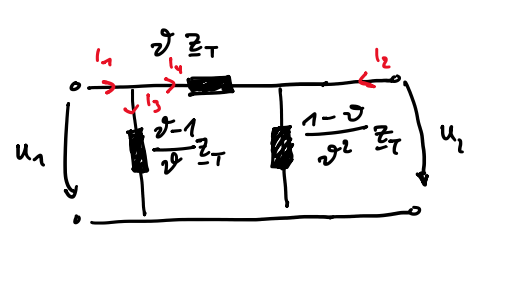
\includegraphics[width=.7\textwidth]{fundamentals/pi_transformer.png}
    \caption[$\Pi$-representative circuit of a transformer with a longitudinal tap changer]{$\Pi$-representative circuit of a transformer with a longitudinal tap changer; own figure after \autocite{machowskiPowerSystemDynamics2020,burlakinEnhancedVoltageControl2024}}
    \label{fig:pi-transformer}
\end{figure}

\begin{align}
    \underline{I}&=\underline{\mab{Y}} \cdot \underline{U} \notag \\[12pt]
    \begin{bmatrix}
        \underline{I}_1 \\
        \underline{I}_2
    \end{bmatrix}&= 
    \begin{bmatrix}
        \underline{Y}_{11} & \underline{Y}_{12} \\
        \underline{Y}_{21} & \underline{Y}_{22}
    \end{bmatrix} \cdot
    \begin{bmatrix}
        \underline{U}_1 \\
        \underline{U}_2
    \end{bmatrix} \label{eq:admittance}
\end{align}

The admittance matrix of a two port network can be expressed after \textcite{machowskiPowerSystemDynamics2020} as \autoref{eq:admittance}. For the $\Pi$-model of an \acs{OLTC} transformer it is leading to \autoref{eq:admittance-oltc}.
\begin{align}
    \underline{\mab{Y}}_\mathrm{\Pi,T}&= 
    \begin{bmatrix}
        \underline{Y}_\mathrm{T} & -\underline{\vartheta}\underline{Y}_\mathrm{T} \\
        \underline{\vartheta}^*\underline{Y}_\mathrm{T} & -\underline{\vartheta}^*\underline{\vartheta}\underline{Y}_\mathrm{T}
    \end{bmatrix} \label{eq:admittance-oltc}
\end{align}

\subsubsection*{Per unit system specialities}

Reactances and resistances are referred to the base voltage and apparent power of the operational unit, such as the transformer. The power system simulation uses its own base voltage and base apparent power, enabling the use of one single calculation domain. This is done to simplify the calculation and to make the results easily comparable to each other. Hence, the reffered values have to be transformed from the equipment based values to the simulation based values. The relations and conversions are defined as follows.

\commenting{
    Additionally to consider:
    \begin{itemize}
        \item D-q transformations,
        \item Frequency domains: reactances and inductances are dependent and can change with the base frequency,
        \item Torque and power relations.
    \end{itemize}
}

This specialities are considered in the tap changer modeling, thus further information is given in \autocite{machowskiPowerSystemDynamics2020}, Appendix A.

\subsection{Open-Source Power System Simulation tools}

\commenting{
    Some information about other open source python power system simulation tools, such as:
    \begin{itemize}
        \item Pandapower,
        \item TOPS,
        \item ... .
    \end{itemize}
    Build up like a scan (see Georg's thesis).

    BUT: As well including the there used implementation of transformers mathematical background and complexity.
}

%%%%%%%%%%%%%%%%%%%%%%%%%%%%%%%
\section{Control engineering theory}

\subsection{Commonly used on-load tap changer control}

A few basics are in the interest, understanding differences between real world beahavior, or possible ways of building up a \acs{OLTC} transformer control. This control theory difference can be limiting as well for the results and objectives compared to the actual possible control in the field.

\subsubsection{Typical presets are manually set}

The target voltage is typically set from the control room of the grid operator, coming from pre-calculated load flow analysis. This can be set hours before, or even day-ahead with the estimated loads of the grid. This value is set locally for each operating unit subsequently. The control is then operating locally and without further involvement of the grid operator. 

\commenting{Quelle dafür finden?}

\subsubsection{Discrete controllers are used in the field}

Typically the used controller in the field is a discrete controller, which can change tap positions under load within a time frame of around few seconds. Practical tap steps are around $2~\mathrm{\%}$ of the overall transforming ratio. The control is set up with a dead band, to avoid unnecessary tap changes. It is necessecary to note here, that this control and its mathematical caracteristics contains logical elements, blocks, and delays, which cannot be translated in a typical control theory transmission function. This leads to the missing possibility to easily obtain mathematical stability for the control of the overall considered power system.

\commenting{Quelle dafür finden?}

\subsection{Dynamic voltage stability}

\commenting{
    Can I really express this as \glqq Controller theory\grqq?
}

\subsection{Bifurcations and Chaos theory control}

\commenting{
    \begin{enumerate}
        \item Fuzzy Control mechanisms,
        \item Neural Networks,
        \item Bifurcations.
\end{enumerate}
}